\documentclass[conference]{IEEEtran}
\IEEEoverridecommandlockouts

\usepackage{cite}
\usepackage{amsmath,amssymb,amsfonts,amsthm}
\usepackage{algorithm}
\usepackage{algpseudocode}
\usepackage{graphicx}
\usepackage{textcomp}
\usepackage{xcolor}
\usepackage{booktabs}
\usepackage{url}
\usepackage[hidelinks]{hyperref}

% Definitions, remarks and assumptions are set upright: they carry long explanatory
% paragraphs, and a page of italics is hard to read. Statements that are claimed to be
% true (propositions) stay italic so they stand out from the prose around them.
\theoremstyle{plain}
\newtheorem{proposition}{Proposition}
\theoremstyle{definition}
\newtheorem{definition}{Definition}
\newtheorem{remark}{Remark}
\newtheorem{assumption}{Assumption}

% "In words": the plain-language reading of the formal statement just made. Every symbol
% introduced in a definition is explained here the first time it appears.
\newcommand{\inwords}{\par\smallskip\noindent\textit{In words.}\ }

\newcommand{\R}{\mathbb{R}}
\newcommand{\N}{\mathbb{N}}
\newcommand{\W}{\mathcal{W}}
\newcommand{\Obs}{\mathcal{O}}
\newcommand{\Rob}{\mathcal{R}}
\newcommand{\Cand}{\mathcal{C}}
\newcommand{\Bod}{\mathcal{B}}
\newcommand{\X}{\mathcal{X}}
\newcommand{\Uc}{\mathcal{U}}
\newcommand{\Core}{\mathcal{K}}
\newcommand{\clr}{\varepsilon}

\begin{document}

\title{Unsatisfiability as a Coordination Signal:\\
Core-Guided Resampling for Multi-Robot\\
Kinodynamic Motion Planning}

% TODO: fill in the author block before submission. Square brackets must stay braced
% here -- a bare [ after \\ is parsed as the optional length argument of \\.
\author{\IEEEauthorblockN{{Author Name}}
\IEEEauthorblockA{\textit{{Department}} \\
\textit{{Institution}} \\
{City, Country} \\
{email@institution.edu}}
}

\maketitle

\begin{abstract}
Multi-robot kinodynamic planners resolve inter-robot conflicts reactively: a collision is
observed between two specific trajectories, and that pair is re-planned. The trigger is an
\emph{instance} of failure. We replace it with a \emph{proof}. Each robot owns a growing
finite set of candidate motions, built with standard components --- a geometric RRT path,
corner smoothing, a speed profile, and execution through the robot's own dynamics --- so
that each candidate is drivable by construction. A SAT solver selects one candidate per
robot, and pairwise collision clauses are added lazily, only for the combinations the solver
actually proposes. When the solver reports \textsc{unsat}, its \emph{unsatisfiable core}
certifies that the current candidate sets admit no collision-free selection, and it names
the robots responsible and the workspace points where their candidates meet. That
certificate drives repair: only the named robots are resampled, with virtual obstacles
placed on the contested points so the sampler is pushed out of the corridor that failed.
The same clause database then certifies the makespan: bisecting a horizon cap over the
candidates already built ends with an \textsc{unsat} proof that no shorter selection
exists. We give every definition, carry a four-robot instance through every step with the
numbers the implementation produces (three rounds, $126$ pairwise checks, a round that
proves a second impasse with zero new geometric work, and a makespan bisected from $698$ to
a certified $353$ steps), and report results on $16$- and $32$-robot benchmark scenarios.
\end{abstract}

\begin{IEEEkeywords}
multi-robot systems, kinodynamic motion planning, satisfiability, conflict resolution
\end{IEEEkeywords}

\section{Introduction}

A multi-robot kinodynamic planner has to answer two questions of different kinds. The first
is continuous --- \emph{what motion can robot $i$ execute?} --- and is answered by machinery
that knows about acceleration bounds, turning limits and obstacles. The second is
combinatorial --- \emph{which motions do the robots execute together?} --- and is answered by
machinery that knows about mutual exclusion. Most planners in this space, including K-ARC
\cite{karc2025}, db-CBS \cite{dbcbs2024} and db-LaCAM \cite{dblacam2025}, answer the second
question by repeatedly re-asking the first: a conflict is found, a constraint is imposed,
and a continuous planner is invoked again.

This paper changes what the combinatorial layer is allowed to say back. In a
conflict-driven planner the signal is always ``\emph{these two trajectories touch}'' --- a
statement about one observed failure. A solver working over a finite set of candidates can
say something strictly stronger: ``\emph{no selection from these candidates works, and here
is the subset of refutations that already makes it impossible}''. That is a statement about
the \emph{entire} candidate set, and it comes at no extra cost: it is what a modern SAT
solver returns when it proves unsatisfiability under tracked assertions \cite{z3}.

We deliberately keep everything else standard. Candidate motions are built from a geometric
RRT \cite{lavalle2001}, a shortcut pass, Gaussian corner smoothing, a forward--backward speed
profile and a tracking rollout through the robot's own integrator. None of these components
is new, and we do not claim them. The contribution is the loop that connects them: what is
resampled, for which robots, and where, is decided by an unsatisfiable core rather than by a
collision, a priority order or a random restart.

\subsection*{Contributions}

\begin{enumerate}
  \item A formulation in which coordination is a Boolean selection problem over per-robot
        candidate sets, with collision clauses added lazily and tracked, so that
        unsatisfiability yields a core (Sec.~\ref{sec:encoding}).
  \item A repair operator driven by that core: the robots it names are resampled around
        virtual obstacles placed on the contested points it names, and are offered a
        longer en-route wait on their existing path (Sec.~\ref{sec:repair}).
  \item A makespan certificate from the same machinery: horizon bisection over the cached
        clauses terminates with a proof that no shorter selection exists among the
        candidates built (Sec.~\ref{sec:bisect}, Prop.~\ref{prop:bisect}).
  \item A fully worked four-robot instance with the implementation's actual numbers
        (Sec.~\ref{sec:example}), measurements justifying each standard component we use
        (Sec.~\ref{sec:design}), and results on benchmark scenarios with up to $32$ robots
        (Sec.~\ref{sec:experiments}).
\end{enumerate}

\section{Related Work}

\paragraph*{Conflict-driven multi-robot planning}
Conflict-Based Search \cite{cbs2015} established the two-level pattern: a low level plans
for one agent, a high level branches on an observed conflict. db-CBS \cite{dbcbs2024} and
db-LaCAM \cite{dblacam2025} carry it into kinodynamic settings by composing
discontinuity-bounded motion primitives. K-ARC \cite{karc2025} builds a sub-problem around
each conflicting \emph{pair} and grows it when resolving one conflict spoils another. In all
of these the unit of blame is a pair of trajectories that were observed to touch. Prioritized
planning \cite{erdmann1987} avoids blame altogether by fixing an order in advance.

\paragraph*{SAT and SMT encodings}
Surynek \cite{surynek2020} gives the closest methodological precedent: a lazy SMT encoding
for continuous multi-agent path finding, in which collision constraints are added on demand.
The difference is what happens on \textsc{unsat}. In \cite{surynek2020} the candidate
structure is a fixed roadmap, so unsatisfiability under a makespan bound is resolved by
raising the bound. Here the candidate sets are themselves refined, so unsatisfiability is a
statement about the \emph{motions we generated}, and the core says which of them to
regenerate.

\paragraph*{Trajectory realisation}
Differential flatness has been used to avoid boundary-value problems in trajectory
generation since \cite{mellinger2011}. Time-optimal path parameterisation under actuator
bounds has a modern reachability-based treatment in TOPP-RA \cite{toppra2018}; we use the
simpler forward--backward sweep. Path smoothing for car-like robots is surveyed together
with its curvature considerations in \cite{elbanhawi2015}. For continuous-time inter-robot
safety, Park and Kim \cite{parkkim2020} certify pairs of polynomial trajectories through
their relative Bernstein coefficients; we return to this in Sec.~\ref{sec:properties}.

\section{Preliminaries}
\label{sec:prelim}

This section fixes every object the method uses. Table~\ref{tab:notation} collects the
notation in one place so that it can be consulted while reading later sections; each symbol
is also explained in words where it is first defined.

\begin{table*}[t]
\caption{Notation. Symbols are grouped by where they are introduced.}
\label{tab:notation}
\centering
\small
\begin{tabular}{@{}l l@{\hspace{2.5em}}l l@{}}
\toprule
\multicolumn{2}{@{}l}{\textbf{World and robots} (Sec.~\ref{sec:prelim-world})} &
\multicolumn{2}{l@{}}{\textbf{Candidates} (Sec.~\ref{sec:prelim-paths}--\ref{sec:prelim-topp})} \\
$\W,\ \Obs$ & workspace; set of static obstacles &
$\gamma_i$ & guide polyline for robot $i$ (RRT output) \\
$N,\ \Rob=\{0,\dots,N{-}1\}$ & number of robots; robot indices &
$L$ & arclength of a curve [m] \\
$A_i,\ \Bod_i(p)$ & body shape; region it occupies at pose $p$ &
$\sigma$ & Gaussian blur length [m] \\
$q=(x,y,\theta,v,\omega)$ & state: position, heading, speeds &
$\sigma_0,\ \delta_{\max}$ & base blur; allowed deviation from the guide [m] \\
$u=(a,\alpha)$ & control: linear, angular acceleration &
$\kappa(s)$ & signed curvature at arclength $s$ [1/m] \\
$\Phi_i,\ \Delta t$ & one-step integrator; time step ($0.1$\,s) &
$\bar v(s)$ & speed profile along the curve [m/s] \\
$\tau_i,\ |\tau_i|$ & executed trajectory; its length in steps &
$\lambda$ & time-scale factor ($\lambda \ge 1$ = slower) \\
$r^{+}_i,\ r^{-}_i$ & bounding, inscribed radius of $A_i$ &
$\chi,\ w$ & wait position (fraction of path); wait length [steps] \\
\cmidrule(r{2.5em}){1-2}\cmidrule(l){3-4}
\multicolumn{2}{@{}l}{\textbf{Collision} (Sec.~\ref{sec:prelim-collision})} &
\multicolumn{2}{l@{}}{\textbf{Solver and repair} (Sec.~\ref{sec:prelim-sat}, \ref{sec:method})} \\
$\clr$ & required surface clearance ($0.05$\,m) &
$\Cand_i,\ \tau_i^{(c)}$ & candidate set of robot $i$; its $c$-th element \\
$d_{\text{surf}}$ & distance between two bodies' surfaces &
$x_{i,c}$ & Boolean: ``robot $i$ executes candidate $c$'' \\
$\xi(\tau_i,\tau_j)$ & first contact point, or $\bot$ if none &
$\ell_{i,c,j,c'}$ & tracking literal of one learned clause \\
\cmidrule(r{2.5em}){1-2}
\multicolumn{2}{@{}l}{\textbf{Problem} (Sec.~\ref{sec:problem})} &
$\Gamma$ & learned clause database \\
$g_i,\ \varrho$ & goal position; goal tolerance radius &
$\Core$ & unsatisfiable core (set of tracking literals) \\
$T,\ T_{\max}$ & plan length; horizon budget [steps] &
$\beta,\ H_i$ & blame map; contested points it assigns to robot $i$ \\
 & &
$b$ & virtual obstacle radius, $2\max_j r^{+}_j + \clr$ \\
 & &
$h$ & horizon cap used during bisection [steps] \\
\bottomrule
\end{tabular}
\end{table*}

\subsection{Workspace, bodies and robots}
\label{sec:prelim-world}

\begin{definition}[Workspace and obstacles]
The workspace is a bounded planar region $\W \subset \R^2$. A finite set
$\Obs = \{o_1,\dots,o_M\}$ of static obstacles is given, each $o_m \subset \W$ a closed
convex set (in our instances, axis-aligned rectangles).
\inwords
$\W$ is the floor the robots drive on --- a $17 \times 17$\,m square in every instance of
this paper --- and $\Obs$ is the list of things on that floor they must not touch. $M$ is
simply how many such things there are; $M = 0$ is an empty room.
\end{definition}

\begin{definition}[Pose and occupancy]
A \emph{pose} is a triple $p = (x,y,\theta)$: a position in the plane and a heading angle.
Robot $i$ has a rigid body $A_i \subset \R^2$, a closed convex polygon described in the
robot's own frame. Its \emph{occupancy} at pose $p$ is
\[
  \Bod_i(p) \;=\; \{\, R(\theta)\,z + (x,y)^{\!\top} \;:\; z \in A_i \,\},
\]
with $R(\theta)$ the rotation matrix by angle $\theta$.
\inwords
$A_i$ is the shape of the robot drawn once, centred at the origin and facing along the
$x$-axis. $\Bod_i(p)$ is that same shape after it has been rotated by $\theta$ and moved to
$(x,y)$: the patch of floor the robot covers when it stands at pose $p$. The formula just says
``rotate every point $z$ of the shape, then shift it''. In our instances $A_i$ is a
$0.5 \times 0.25$\,m box, so heading matters: a box sideways in a corridor needs more room
than a box end-on.
\end{definition}

\begin{definition}[Second-order unicycle]
\label{def:robot}
The robot model is the second-order unicycle with the parameter values published for
\texttt{unicycle2\_v0} in dynobench \cite{dynobench}. Its state and control are
\[
  q = (x,y,\theta,v,\omega) \in \X \subset \R^5,
  \qquad
  u = (a,\alpha) \in \Uc \subset \R^2 ,
\]
and its equations of motion are
\begin{equation}
  \dot x = v\cos\theta,\quad
  \dot y = v\sin\theta,\quad
  \dot\theta = \omega,\quad
  \dot v = a,\quad
  \dot\omega = \alpha ,
  \label{eq:dyn}
\end{equation}
subject to the box bounds
\begin{equation}
  |v| \le v_{\max},\quad |\omega| \le \omega_{\max},\quad
  |a| \le a_{\max},\quad |\alpha| \le \alpha_{\max},
  \label{eq:bounds}
\end{equation}
with $v_{\max}=0.5$\,m/s, $\omega_{\max}=0.5$\,rad/s, $a_{\max}=0.25$\,m/s$^2$ and
$\alpha_{\max}=0.25$\,rad/s$^2$ for every robot in this paper.
\inwords
The robot drives forward along its heading at speed $v$ and turns at rate $\omega$. What
makes it \emph{kinodynamic} rather than kinematic is that $v$ and $\omega$ are part of the
state $q$, not inputs: the planner can only choose the accelerations $a$ (speed up / slow
down) and $\alpha$ (start / stop turning). The robot therefore has momentum --- it cannot
stop or change direction instantly --- and \eqref{eq:bounds} caps how fast it may go and how
hard it may accelerate. $\X$ and $\Uc$ are just names for ``all states'' and ``all controls
within those bounds''.
\end{definition}

\begin{remark}[Two derived constants]
The bounds fix two lengths that recur throughout. The \emph{braking distance} from full
speed is $d_{\text{brake}} = v_{\max}^2/(2a_{\max}) = 0.50$\,m: a robot at full speed needs
half a metre to stop. The \emph{minimum turning radius} at full speed is
$\rho = v_{\max}/\omega_{\max} = 1.00$\,m: to turn tighter than that, the robot must slow
down. Both are large compared with the body ($0.5$\,m long) and the goal tolerance
($0.2$\,m), so these problems cannot be solved by ignoring the dynamics.
\end{remark}

\begin{definition}[Executed trajectory]
\label{def:exec}
Time is discretised with step $\Delta t = 0.1$\,s. Let $\Phi_i : \X \times \Uc \to \X$ be the
one-step map obtained by integrating \eqref{eq:dyn} over $\Delta t$ with fourth-order
Runge--Kutta, with $v$ and $\omega$ saturated to their bounds after the step. Given a start
state $q_i^0$ and controls $\mathbf{u}_i = (u_i^0,\dots,u_i^{T-1})$, every $u_i^k \in \Uc$,
the \emph{executed trajectory} is
\[
  \tau_i \;=\; (q_i^1, \dots, q_i^T),
  \qquad q_i^{k+1} = \Phi_i(q_i^k, u_i^k).
\]
We write $p_i^k = (x_i^k, y_i^k, \theta_i^k)$ for the pose part of $q_i^k$ and
$|\tau_i| = T$ for the number of steps.
\inwords
$\Phi_i$ is ``advance the robot by one tenth of a second under control $u$''. The executed
trajectory is what you get by starting at $q_i^0$ and applying the controls one after
another: a list of states, one per time step. The superscript $k$ is always a time index,
never a power. $|\tau_i|$ is how long the motion takes, counted in steps; multiply by
$\Delta t$ for seconds.
\end{definition}

\begin{remark}[Why the executed trajectory is the object of interest]
Everything the planner checks and reports is defined on $\tau_i$ as produced by $\Phi_i$
--- not on a reference curve or a path. A reference the robot does not actually follow would
certify a motion nobody drives. This is why the tracking step of Sec.~\ref{sec:realise} is
part of the planner and not post-processing.
\end{remark}

\subsection{Collision semantics}
\label{sec:prelim-collision}

\begin{definition}[Overlap and surface distance]
Two bodies at poses $p, p'$ \emph{overlap} iff $\Bod_i(p) \cap \Bod_j(p') \neq \emptyset$.
Their \emph{surface distance} is
\[
  d_{\text{surf}}(i,p,\,j,p') \;=\;
  \min_{z \in \Bod_i(p),\, z' \in \Bod_j(p')} \lVert z - z' \rVert_2 .
\]
\inwords
$d_{\text{surf}}$ is the length of the shortest gap between the two robots' outlines --- the
distance you would measure with a ruler between their nearest edges. It is $0$ exactly when
they touch or overlap. For two boxes it is computed exactly (separating-axis test).
\end{definition}

\begin{definition}[Bounding and inscribed radii]
For a body $A_i$, the \emph{bounding radius} $r^{+}_i = \max_{z \in A_i}\lVert z\rVert$ is
the radius of the smallest origin-centred disc containing it, and the \emph{inscribed
radius} $r^{-}_i$ is the radius of the largest origin-centred disc contained in it. For a
$w \times \ell$ box, $r^{+} = \tfrac12\sqrt{w^2+\ell^2}$ and $r^{-} = \tfrac12\min(w,\ell)$;
for our robots $r^{+} = 0.2795$\,m and $r^{-} = 0.125$\,m.
\inwords
$r^{+}$ is the radius of a coin that covers the whole robot however it is rotated;
$r^{-}$ is the radius of the largest coin that fits inside it. They bracket the true shape
from outside and inside, and the next proposition uses exactly that.
\end{definition}

\begin{proposition}[Three-band test]
\label{prop:bands}
Let $\delta = \lVert (x,y) - (x',y') \rVert_2$ be the distance between two robot centres and
$\clr \ge 0$ a clearance threshold. Then
\begin{align}
  \delta \;\ge\; r^{+}_i + r^{+}_j + \clr
    &\;\Longrightarrow\; d_{\text{surf}} \ge \clr, \label{eq:band-far}\\
  \delta \;<\; r^{-}_i + r^{-}_j + \clr
    &\;\Longrightarrow\; d_{\text{surf}} < \clr. \label{eq:band-near}
\end{align}
\end{proposition}

\begin{proof}
Both bodies lie inside their bounding discs, so
$d_{\text{surf}} \ge \delta - r^{+}_i - r^{+}_j$, giving \eqref{eq:band-far}. Both contain
their inscribed discs, so $d_{\text{surf}} \le \delta - r^{-}_i - r^{-}_j$, giving
\eqref{eq:band-near}.
\end{proof}

\begin{remark}[Why this matters computationally]
Prop.~\ref{prop:bands} splits every centre distance into three bands. Far apart
($\delta \ge 0.609$\,m for our robots): certainly clear. Very close ($\delta < 0.300$\,m):
certainly too close. Only in the ring between is the exact box-to-box distance needed. Most
time steps of most pairs are in the far band, and a centre distance is one subtraction, so
checking a pair of long trajectories costs little more than a vector norm.
\end{remark}

\begin{definition}[Pairwise conflict and first contact]
\label{def:conflict}
Two executed trajectories $\tau_i,\tau_j$ \emph{conflict} iff there is a step $k$ with
$d_{\text{surf}}(i,p_i^k,\,j,p_j^k) < \clr$, where the shorter trajectory is held at its
final state for all $k$ beyond its own length. For the least such $k^\ast$, the \emph{first
contact} is the midpoint of the two centres,
\begin{equation}
  \xi(\tau_i,\tau_j) \;=\; \tfrac12\!\left( (x_i^{k^\ast},y_i^{k^\ast}) +
                                            (x_j^{k^\ast},y_j^{k^\ast}) \right),
  \label{eq:xi}
\end{equation}
and $\xi = \bot$ (``no contact'') if no such step exists.
\inwords
Play both motions side by side on the same clock. If at any step the robots come closer than
$\clr = 5$\,cm, they conflict, and $\xi$ is the spot on the floor between them at the first
such moment. $\xi$ is the only piece of geometry the repair step will ever see: it answers
``\emph{where} did these two meet?''.
\end{definition}

\begin{remark}[Holding the final state is not a convenience]
A robot that arrives early stays on its goal, and a parked robot still blocks. Stopping the
comparison when the shorter motion ends would approve plans that drive through a parked
robot.
\end{remark}

\subsection{Geometric paths: RRT and shortcutting}
\label{sec:prelim-paths}

\begin{definition}[Geometric RRT]
\label{def:rrt}
Given a start $s$, a goal $g$, and a disc of radius $r$ standing in for the robot, a
\emph{rapidly-exploring random tree} \cite{lavalle2001} grows a tree of collision-free
positions from $s$. Each iteration draws a target --- the goal with probability $p_g$,
otherwise a uniformly random point of $\W$ --- finds the nearest tree node, and adds a new
node at most $\eta$ metres towards the target if that node and the segment to it keep the
disc clear of $\Obs$ and inside $\W$. It stops when a node within $\eta$ of $g$ can see $g$,
and returns the tree path from $s$ to $g$ as a polyline $\gamma$.
\inwords
Throw random darts at the map; each time, extend the nearest branch of the tree a short step
($\eta = 0.6$\,m) towards the dart, as long as the step does not hit anything. One dart in
ten ($p_g = 0.1$) is aimed at the goal, which pulls the tree in the right direction. The
robot is treated as a disc of radius $r = r^{+}_i + \clr$ --- the coin that covers it at any
heading, plus clearance --- so the path is safe regardless of which way the robot faces.
The result $\gamma$ is a list of points joined by straight segments: a \emph{path}, with no
notion of time or speed.
\end{definition}

\begin{definition}[Shortcutting]
\label{def:shortcut}
Given a polyline $\gamma = (\gamma_0,\dots,\gamma_n)$, a \emph{shortcut} step picks two
vertices $\gamma_a, \gamma_b$ with $b \ge a+2$ at random and, if the straight segment between
them is collision-free for the disc, deletes every vertex strictly between them. We apply
$200$ such steps.
\inwords
An RRT path zig-zags, because it was grown towards random darts. Shortcutting repeatedly
asks ``can I go straight from here to there instead?'' and, when the answer is yes, cuts
out the detour. Because it only ever deletes vertices, the shortened path stays in the same
corridor the RRT found. On the worked instance a $38$-vertex RRT path collapses to a single
straight segment (Fig.~\ref{fig:worked}(a)).
\end{definition}

\subsection{From a polyline to a drivable curve}
\label{sec:prelim-smooth}

A polyline has corners, and a corner is a point of infinite curvature. The robot cannot
drive through one at any speed (Prop.~\ref{prop:caps} below), so the corners are rounded
first.

\begin{definition}[Gaussian path smoothing]
\label{def:blur}
Resample $\gamma$ at $600$ points spaced evenly by arclength, with spacing $\Delta s$.
Convolve the $x$- and $y$-coordinate sequences separately with a Gaussian kernel of standard
deviation $\sigma/\Delta s$ samples, padding both ends by \emph{linear extrapolation} of the
first and last segments. Resample the result evenly by arclength again. We call the result
the curve $\gamma^{\sigma}$ and $\sigma$ (in metres) its \emph{blur length}.
\inwords
Replace every point of the path by a weighted average of its neighbours within roughly
$\sigma$ metres. Straight stretches stay exactly where they are (the average of points on a
line is on the line); corners get rounded, more so for larger $\sigma$. The padding detail
matters: padding by repeating the end point would pull the first and last points inwards,
i.e.\ move the start and the goal. Extrapolating the end segments leaves them in place.
\end{definition}

\begin{definition}[Deviation and largest admissible blur]
\label{def:fitblur}
The \emph{deviation} of $\gamma^{\sigma}$ from $\gamma$ is
$\operatorname{dev}(\sigma) = \max_{z \in \gamma^{\sigma}} \min_{z' \in \gamma}
\lVert z - z'\rVert$, evaluated against a densely resampled $\gamma$. Given a base blur
$\sigma_0$ and a tolerance $\delta_{\max}$, the \emph{chosen blur} is
\begin{equation}
\begin{aligned}
  \sigma^\ast = \max\big\{\, \sigma \in \{8,4,2,1\}\cdot\sigma_0 \;:\;
    &\operatorname{dev}(\sigma) \le \delta_{\max},\\
    &\gamma^{\sigma} \text{ clears } \Obs \,\big\},
\end{aligned}
  \label{eq:fitblur}
\end{equation}
or $\sigma_0$ if the set is empty. We use $\sigma_0 = 0.12$\,m and
$\delta_{\max} = \tfrac12(2r^{+}_i + \clr) = 0.30$\,m.
\inwords
Round the corners as much as possible, but not so much that the curve wanders more than
$30$\,cm (about half a robot width) from the path the RRT found, and never into an obstacle.
The check is made for body poses along the curve, with heading taken from the curve itself,
since a box swung around a corner sweeps more than its disc suggests. Four blur lengths are
tried, largest first ($0.96, 0.48, 0.24, 0.12$\,m). The reason to prefer the largest is
speed: gentler corners can be taken faster (Prop.~\ref{prop:caps}), and
Sec.~\ref{sec:design} shows the effect is large.
\end{definition}

\begin{definition}[Arclength, heading, curvature]
On the evenly spaced curve $\gamma^{\sigma^\ast} = (z_0,\dots,z_{599})$ with spacing
$\Delta s$, the station of $z_k$ is $s_k = k\Delta s$, its heading is
$\theta(s_k) = \operatorname{atan2}(y'_k, x'_k)$, and its signed curvature is
\[
  \kappa(s_k) \;=\; \frac{x'_k\, y''_k - y'_k\, x''_k}{\big(x'^2_k + y'^2_k\big)^{3/2}},
\]
with derivatives with respect to arclength taken by central finite differences.
\inwords
$s$ measures distance travelled along the curve, from $0$ at the start to $L$ at the goal.
$\theta(s)$ is the direction the curve points at station $s$. $\kappa(s)$ is how sharply it
bends there: $0$ on a straight line, $1/R$ on a circle of radius $R$, positive for left
turns and negative for right turns.
\end{definition}

\subsection{Differential flatness: why no boundary-value problem}
\label{sec:prelim-flat}

\begin{definition}[Differential flatness]
A system $\dot q = f(q,u)$ is \emph{differentially flat} with \emph{flat output} $\phi$ if
the full state $q$ and control $u$ can be written as algebraic functions of $\phi$ and
finitely many of its time derivatives.
\inwords
There is a small set of quantities $\phi$ such that, once you have decided how $\phi$
evolves over time, everything else --- every state variable and every control --- follows by
differentiation, with no equation left to solve. Choosing $\phi(t)$ \emph{is} choosing a
trajectory.
\end{definition}

\begin{proposition}[Flatness of \eqref{eq:dyn}]
\label{prop:flat}
System \eqref{eq:dyn} is flat with flat output $\phi = (x,y)$. For any twice-differentiable
curve traversed with nonzero speed,
\begin{equation}
\begin{aligned}
  \theta &= \operatorname{atan2}(\dot y, \dot x), & v &= \sqrt{\dot x^2 + \dot y^2},\\
  \omega &= \kappa\, v, & a &= \dot v, \quad \alpha = \dot\omega .
\end{aligned}
  \label{eq:flatmap}
\end{equation}
\end{proposition}

\begin{proof}
From \eqref{eq:dyn}, $(\dot x,\dot y) = v(\cos\theta,\sin\theta)$, so $v$ is the speed and
$\theta$ the direction of motion wherever $v \ne 0$. Differentiating $\theta$ and using the
curvature formula gives $\dot\theta = \kappa v$, which is $\omega$. The controls are the
time derivatives of $v$ and $\omega$.
\end{proof}

\begin{remark}[Flatness is a closed-form steering function]
\label{rem:steer}
A kinodynamic RRT that grows a tree by sampling controls \cite{lavalle2001} has no way to
\emph{aim} at a given state: connecting two states exactly is a two-point boundary-value
problem, which has no closed-form solution for \eqref{eq:dyn}. Flatness is the reason we do
not need one. We search for a \emph{path} in the plane, where connecting two points is a
straight line, and Prop.~\ref{prop:flat} turns any smooth path plus a speed profile into
states and controls. What flatness does \emph{not} provide is \eqref{eq:bounds}; those depend
on how fast the curve is traversed, and are imposed next. Note also that \eqref{eq:flatmap}
needs $v \ne 0$: heading is undefined for a robot at rest, which is why the rollout in
Sec.~\ref{sec:realise} begins by turning on the spot.
\end{remark}

\subsection{Speed profiles and time scaling}
\label{sec:prelim-topp}

\begin{definition}[Speed profile]
A \emph{speed profile} on a curve of length $L$ is a function $\bar v : [0,L] \to \R_{\ge 0}$
giving the forward speed at each station $s$. It fixes the time at which each station is
reached, $t(s) = \int_0^s \bar v(\bar s)^{-1} d\bar s$.
\inwords
The curve says \emph{where} the robot goes; $\bar v(s)$ says \emph{how fast} it is going when
it passes station $s$. Together they are a complete timed motion. The bar distinguishes the
profile, a function of distance, from the state variable $v$, a function of time.
\end{definition}

\begin{proposition}[Pointwise speed caps]
\label{prop:caps}
Under \eqref{eq:flatmap}, $|v| \le v_{\max}$ and $|\omega| \le \omega_{\max}$ hold everywhere
iff
\begin{equation}
  \bar v(s) \;\le\; \min\!\left( v_{\max},\; \frac{\omega_{\max}}{|\kappa(s)|} \right)
  \quad \text{for all } s .
  \label{eq:vlim}
\end{equation}
\end{proposition}

\begin{proof}
Immediate from $\omega = \kappa v$.
\end{proof}

\begin{remark}[The turning-speed coupling]
Eq.~\eqref{eq:vlim} says: on a bend of radius $R = 1/|\kappa|$, the robot may go no faster
than $\omega_{\max} R$. On our robots a bend of radius $0.5$\,m allows only $0.25$\,m/s ---
half the top speed. One sharp corner therefore slows the robot for the whole stretch around
it, and this is precisely what the largest-blur rule \eqref{eq:fitblur} is buying back.
\end{remark}

The acceleration bound couples neighbouring stations (you cannot be at $0$\,m/s at one
station and $0.5$\,m/s ten centimetres later). On the grid $s_0 < \dots < s_{599}$ it is
enforced by two sweeps, starting from the caps \eqref{eq:vlim} with $\bar v_0 = \bar v_{599} = 0$:
\begin{align}
  \text{forward: } \; & \bar v_{k+1} \leftarrow \min\!\big(\bar v_{k+1},\, \sqrt{\bar v_k^2 + 2 a_{\max}\Delta s}\big),
  \label{eq:fwd}\\
  \text{backward: } \; & \bar v_{k} \leftarrow \min\!\big(\bar v_{k},\, \sqrt{\bar v_{k+1}^2 + 2 a_{\max}\Delta s}\big).
  \label{eq:bwd}
\end{align}
In words: the forward sweep says you cannot arrive at a station faster than you could have
accelerated to from the previous one; the backward sweep says you cannot carry more speed
into a station than you could brake off before the next. Both only \emph{lower} speeds, so
\eqref{eq:vlim} still holds afterwards. This is the classical construction; TOPP-RA
\cite{toppra2018} is a stronger modern treatment.

The last bound, $|\alpha| \le \alpha_{\max}$, involves how fast curvature changes along the
curve, and is cleared by slowing the whole motion down uniformly.

\begin{proposition}[Time scaling]
\label{prop:scale}
Let $\tau$ be a trajectory of \eqref{eq:dyn} and $\lambda \ge 1$. Traversing the same path
with $t \mapsto t/\lambda$ gives
\[
  v \mapsto v/\lambda, \quad \omega \mapsto \omega/\lambda, \quad
  a \mapsto a/\lambda^2, \quad \alpha \mapsto \alpha/\lambda^2 ,
\]
and leaves the geometric path, and therefore $\kappa$ and obstacle clearance, unchanged.
\end{proposition}

\begin{proof}
Differentiate $\phi(t/\lambda)$ once and twice.
\end{proof}

\begin{remark}[Two uses of time scaling]
\label{rem:scale}
$\lambda$ is a ``slow-motion factor'': $\lambda = 2$ plays the same motion at half speed,
taking twice as long. First, it repairs $\alpha$: if the worst ratio of an acceleration to
its bound is $\mu > 1$, dividing the profile by $\sqrt{\mu}$ brings it to $1$; we iterate
this up to six times. Second, it gives the coordination layer a free alternative: the same
path at a slower pace is guaranteed to satisfy every bound the fast one did, and to be just
as clear of obstacles.
\end{remark}

\subsection{Satisfiability, cores and lazy refinement}
\label{sec:prelim-sat}

\begin{definition}[Propositional satisfiability]
Given Boolean variables and a formula $F$ built from them, the SAT problem asks for a true /
false assignment $\mu$ that makes $F$ true (written $\mu \models F$), or a proof that none
exists. We use z3 \cite{z3}, which also accepts cardinality constraints such as ``exactly
one of these variables is true'' directly.
\inwords
A SAT solver takes a list of yes/no questions with logical rules connecting them, and
either returns answers satisfying every rule (\textsc{sat}) or proves that no such answers
exist (\textsc{unsat}).
\end{definition}

\begin{definition}[Tracked assertion and unsatisfiable core]
\label{def:core}
A \emph{tracked} assertion attaches a fresh Boolean \emph{tracking literal} $\ell$ to a
clause $\phi$, asserting $\ell \rightarrow \phi$ with $\ell$ assumed true. If the formula is
unsatisfiable, the solver returns an \emph{unsatisfiable core} $\Core$: a subset of the
tracking literals whose clauses, together with the untracked part of the formula, are
already unsatisfiable.
\inwords
Give every rule a name tag. When the solver says ``impossible'', ask it \emph{which} tags it
used to prove that. The answer, $\Core$, is a list of rules that are already contradictory
among themselves --- the part of the problem that is actually responsible, with the rest
set aside.
\end{definition}

\begin{remark}[What a core is and is not]
A core is a \emph{sufficient} explanation, not necessarily the smallest: solvers return a
small core, not a minimum one. Used as blame, it may therefore occasionally name a robot a
cleverer explanation would have spared. Every rule it names, however, is a genuine
refutation --- nothing in a core is invented.
\end{remark}

\begin{definition}[Lazy refinement (CEGAR)]
\label{def:cegar}
A constraint that is expensive to write out in full is added \emph{lazily}: the solver is
queried without it, the proposed assignment is tested by an \emph{oracle}, and if the test
fails a clause forbidding that failure is added and the solver is queried again. The loop
ends when the oracle accepts, or the solver reports \textsc{unsat}.
\inwords
Do not tell the solver about every possible collision up front --- there are far too many.
Let it guess, check the guess, and teach it only the collisions its guesses actually run
into. This is counterexample-guided abstraction refinement; \cite{surynek2020} uses it for
continuous multi-agent path finding.
\end{definition}

\section{Problem Statement}
\label{sec:problem}

\begin{definition}[Instance]
\label{def:instance}
An instance is a tuple
$\big(\W, \Obs, \Rob, \{A_i\}, \{q_i^{0}\}, \{g_i\}, \Delta t, T_{\max}, \clr, \varrho\big)$,
where $\Rob = \{0,\dots,N-1\}$ indexes the robots, $q_i^{0} \in \X$ is robot $i$'s start
state (at rest), $g_i \in \R^2$ its goal position, $T_{\max}$ a horizon budget in steps,
$\clr > 0$ the required surface clearance, and $\varrho$ the goal tolerance.
\inwords
Everything that is given: the room, the obstacles, which robots exist and what shape they
are, where each starts and where each must go, the clock tick, how long the plan may take at
most, how close robots may come to one another, and how close to its goal a robot must stop
to count as arrived.
\end{definition}

\begin{definition}[Admissible plan]
\label{def:plan}
A \emph{plan} is a tuple of control sequences $(\mathbf{u}_0,\dots,\mathbf{u}_{N-1})$ padded
to a common length $T$ (a finished robot receives zero controls), inducing executed
trajectories $\tau_i$ by Def.~\ref{def:exec}. It is \emph{admissible} iff:
\begin{enumerate}
  \item[(P1)] \textbf{Control bounds.} $u_i^k \in \Uc$ for all $i,k$.
  \item[(P2)] \textbf{Obstacle freedom.} $\Bod_i(p_i^k) \cap o = \emptyset$ for all
        $i$, all $k \le T$ and all $o \in \Obs$.
  \item[(P3)] \textbf{Mutual clearance.}
        $d_{\text{surf}}(i,p_i^k,\,j,p_j^k) \ge \clr$ for all $i < j$ and all $k \le T$.
  \item[(P4)] \textbf{Goal arrival.}
        $\lVert (x_i^T,y_i^T) - g_i \rVert_2 < \varrho$ for every $i$.
  \item[(P5)] \textbf{Horizon.} $T \le T_{\max}$.
\end{enumerate}
\inwords
(P1): the robot can actually produce the commanded accelerations. (P2): no robot ever touches
an obstacle. (P3): no two robots ever come within $\clr$ of each other. (P4): at the end,
every robot is within $\varrho$ of its goal. (P5): the whole thing finishes in time.
\end{definition}

\begin{definition}[Problem]
\label{def:problem}
Given an instance, find an admissible plan with small \emph{makespan} $T\Delta t$ --- the time
at which the last robot has finished --- or report failure.
\end{definition}

\begin{remark}[Discrete-time semantics]
(P2) and (P3) are required at the time steps $k$, not at every instant in between. This is
the semantics under which the simulator scores collisions, so it is what a plan must satisfy
to be honest about what the simulator will report. It is \emph{not} a continuous-time
guarantee; Remark~\ref{rem:gap} states what is left open.
\end{remark}

\begin{assumption}
\label{ass:homog}
For clarity, all robots in this paper share one model and one body. Nothing in the method
requires it: every bound is read from robot $i$'s own model, and Def.~\ref{def:conflict} is
already per pair in both bodies and radii.
\end{assumption}

\section{Method}
\label{sec:method}

\subsection{Overview}

The method keeps, for each robot $i$, a finite and only-growing \emph{candidate set}
\[
  \Cand_i \;=\; \{\,\tau_i^{(0)}, \tau_i^{(1)}, \dots\,\}
\]
of executed trajectories from $q_i^0$ towards $g_i$. The superscript $(c)$ is a candidate
index, not a time step. Each candidate is built for robot $i$ alone and knows nothing about
the others. Coordination is then the discrete question of picking one element from each
$\Cand_i$ so that no two picks conflict. One \emph{round} of the loop is:

\begin{enumerate}
  \item \textbf{Select.} Ask z3 for one candidate per robot, subject to every clause learned
        so far (Sec.~\ref{sec:encoding}).
  \item \textbf{Refute.} Check the selected candidates pairwise (Def.~\ref{def:conflict});
        for each conflicting pair, learn a tracked clause and ask again
        (Sec.~\ref{sec:oracle}). If no pair conflicts, verify and go to step 5.
  \item \textbf{Explain.} When z3 reports \textsc{unsat}, read the core and turn it into a
        blame map from robots to contested points (Sec.~\ref{sec:core}).
  \item \textbf{Repair.} Resample each blamed robot's path around its contested points and
        add the new candidates (Sec.~\ref{sec:repair}); start the next round.
  \item \textbf{Shorten.} Bisect a horizon cap over the same candidates and clauses
        (Sec.~\ref{sec:bisect}), and return the shortest plan found.
\end{enumerate}
Before the first round, every robot is seeded with one sampled path and its variants
(Sec.~\ref{sec:candidates}). Algorithm~\ref{alg:main} states the loop.

\begin{algorithm}[t]
\caption{Core-guided coordination}
\label{alg:main}
\begin{algorithmic}[1]
\Require instance (Def.~\ref{def:instance}), round cap $N_r$, deadline $D$
\Ensure an admissible plan, or \textsc{fail}
\For{$i \in \Rob$}
  \State $\gamma_i^{\text{seed}} \gets \textsc{SampleGuide}(i, \emptyset)$;\quad
         $\Cand_i \gets \textsc{Variants}(i, \gamma_i^{\text{seed}})$
\EndFor
\State $\Gamma \gets \emptyset$ \Comment{learned clauses, never retracted}
\For{$r = 1 \dots N_r$}
  \State $(\pi, \text{verdict}, \beta) \gets \textsc{Search}(\Cand, \Gamma, h=\infty)$
  \State \textbf{if} verdict $=$ \textsc{timeout} \textbf{then return} \textsc{fail}
  \If{verdict $=$ \textsc{sat}}
    \State \Return $\textsc{Bisect}(\pi, \Cand, \Gamma)$
  \EndIf
  \State \textbf{if} $\beta = \emptyset$ \textbf{then} $\beta \gets \{\, i \mapsto \emptyset : i \in \Rob\,\}$
  \For{$(i, H_i) \in \beta$}
    \State $\Cand_i \gets \Cand_i \cup \textsc{Repair}(i, H_i)$ \Comment{Alg.~\ref{alg:repair}}
  \EndFor
\EndFor
\State \Return \textsc{fail}
\Statex
\Function{Search}{$\Cand, \Gamma, h$}
  \State assert $\sum_{c} x_{i,c} = 1$ for each $i$; forbid every $x_{i,c}$ with $|\tau_i^{(c)}| > h$
  \State assert every clause of $\Gamma$, tracked (Def.~\ref{def:core})
  \While{true}
    \State \textbf{if} $\textsc{now}() > D$ \textbf{then return} $(\bot, \textsc{timeout}, \emptyset)$
    \State \textbf{if} $\textsc{check}() = \textsc{unsat}$ \textbf{then break}
    \State $\pi \gets$ model: one candidate index $\pi_i$ per robot
    \State $F \gets \{\,(i,j) : i<j,\ \xi(\tau_i^{(\pi_i)}, \tau_j^{(\pi_j)}) \neq \bot,\ \text{not cached}\,\}$
    \If{$F = \emptyset$}
      \State \textbf{if} \textsc{Verify}$(\pi)$ \textbf{then return} $(\pi,\textsc{sat},\emptyset)$
      \State assert $\bigvee_i \neg x_{i,\pi_i}$ \Comment{untracked}
    \Else
      \State add $\ell_{i,\pi_i,j,\pi_j} \rightarrow (\neg x_{i,\pi_i} \vee \neg x_{j,\pi_j})$ to $\Gamma$
             for each $(i,j) \in F$
    \EndIf
  \EndWhile
  \State \Return $(\bot, \textsc{unsat}, \textsc{Blame}(\textsc{core}()))$
\EndFunction
\end{algorithmic}
\end{algorithm}

\subsection{Candidate construction}
\label{sec:candidates}

\paragraph*{Guide}
\textsc{SampleGuide}$(i, \mathcal{V})$ runs the RRT of Def.~\ref{def:rrt} from robot $i$'s
start to its goal with disc radius $r^{+}_i + \clr$, treating the set $\mathcal{V}$ of
\emph{virtual obstacles} (Sec.~\ref{sec:repair}) as if they were real, and shortcuts the
result (Def.~\ref{def:shortcut}). If no path is found within $5000$ iterations, it retries
with the real obstacles only; if that fails too, it returns the straight segment from start
to goal and lets the rollout and the verifier reject it if it is not drivable. Seeding calls
it with $\mathcal{V} = \emptyset$.

\paragraph*{Variants}
One guide yields up to four candidates, which differ only in \emph{timing}:
\begin{itemize}
  \item the fastest admissible traverse ($\lambda = 1$);
  \item a slowed traverse ($\lambda = 1.6$), legal by Prop.~\ref{prop:scale};
  \item two \emph{en-route wait} variants: the path is cut at a fraction $\chi$ of its
        arclength drawn uniformly from $[0.25, 0.7]$; the robot drives the first part to
        rest, holds for $w$ steps ($w = 30$ and $w = 80$), then drives the rest.
\end{itemize}
The fraction $\chi$ says \emph{where} along the path the robot waits (e.g.\ $\chi = 0.5$ is
halfway), and $w$ says \emph{how long}.

\begin{remark}[Why waits are en route and not at the start]
Holding a robot on its start line is the classic prioritized-planning device, but it needs
the delay to be decided with knowledge of everyone else's timing before anyone moves. An
en-route wait is a real manoeuvre --- a real deceleration, a real restart --- and places the
idle time near where conflicts happen. It costs nothing extra to check: the hold is $w$ copies
of a rest state, which Def.~\ref{def:conflict} treats like any other step.
\end{remark}

\subsection{Realising a candidate}
\label{sec:realise}

\textsc{Drive} turns a guide $\gamma$ into an executed trajectory in four stages.

\begin{enumerate}
  \item \textbf{Smooth.} Choose $\sigma^\ast$ by \eqref{eq:fitblur} and form the curve
        $\gamma^{\sigma^\ast}$ with its arclength grid, heading $\theta(s)$ and curvature
        $\kappa(s)$.
  \item \textbf{Profile.} Apply the caps \eqref{eq:vlim}, then the sweeps
        \eqref{eq:fwd}--\eqref{eq:bwd}, then divide by $\lambda$. Convert to a time-indexed
        reference $(x^k, y^k, \theta^k, v^k, \omega^k)$ sampled every $\Delta t$. If the
        reference's finite-difference $|a|$ or $|\alpha|$ exceeds its bound, rescale per
        Remark~\ref{rem:scale} and repeat (at most six times).
  \item \textbf{Execute.} Starting from the robot's actual state, first rotate on the spot
        to the curve's initial heading (needed because \eqref{eq:flatmap} is singular at
        rest). Then, for each step $k$, apply feedforward from flatness plus a proportional
        correction,
        \begin{align}
          a^k &= \frac{v^{k+1}-v^k}{\Delta t} + k_v\,(v^k - \hat v^k), \label{eq:ff-a}\\
          \alpha^k &= \frac{\omega^{k+1}-\omega^k}{\Delta t}
                      + k_\theta\,(\omega^k - \hat\omega^k)
                      + \frac{0.15\,k_\theta}{\Delta t}\, e_\theta^k, \label{eq:ff-al}
        \end{align}
        clipped into $\Uc$ and passed through $\Phi_i$. Here $\hat v^k,\hat\omega^k$ are
        the robot's \emph{actual} speeds (as opposed to the reference's $v^k,\omega^k$),
        $e_\theta^k$ is the heading error wrapped to $(-\pi,\pi]$, and
        $(k_\theta, k_v) = (1.6, 1.2)$ are gains.
  \item \textbf{Stop.} Brake any residual speed to zero, so every candidate ends at rest.
\end{enumerate}
For an en-route wait variant, stages 1--4 are applied to the part of the path before the cut,
$w$ rest states are appended, and stages 1--4 are applied again from that rest state to the
part after the cut.

\begin{proposition}[What holds for every candidate]
\label{prop:admissible}
Every trajectory in $\Cand_i$ satisfies (P1), and is the true response of $\Phi_i$ to its
controls.
\end{proposition}

\begin{proof}
Every control is clipped into $\Uc$ before being applied, and the states are produced by
$\Phi_i$ itself.
\end{proof}

\begin{remark}[What is \emph{not} guaranteed per candidate, and where it is checked]
Obstacle freedom (P2) is designed in --- the guide clears the obstacles with margin
$r^{+}_i + \clr$, and \eqref{eq:fitblur} rejects blurs that cut into them --- but it is not
\emph{proved} for the executed states, because tracking error is not bounded analytically,
and because the straight-segment fallback of \textsc{SampleGuide} is not checked at all.
Goal arrival (P4) likewise depends on tracking. Rather than make a claim about every
candidate, the method checks (P2), (P4) and (P5) on the \emph{selected} plan, with the
simulator's own routine (Sec.~\ref{sec:verify}). Only (P3), the pairwise property, is left to
the solver.
\end{remark}

\subsection{Boolean encoding}
\label{sec:encoding}

\begin{definition}[Selection variables]
For each robot $i$ and each candidate index $c$, introduce a Boolean $x_{i,c}$.
\inwords
$x_{i,c}$ is true iff robot $i$ executes its $c$-th candidate. On the worked instance, $x_{0,2}$
true means ``robot $0$ drives its seed path and waits $30$ steps on the way''.
\end{definition}

The formula has three parts.

\paragraph*{Exactly one candidate per robot}
\begin{equation}
  \sum_{c\,:\,|\tau_i^{(c)}| \le h} x_{i,c} \;=\; 1,
  \qquad
  x_{i,c} = \text{false} \ \text{ whenever } |\tau_i^{(c)}| > h ,
  \label{eq:exactlyone}
\end{equation}
for every robot $i$. The \emph{horizon cap} $h$ excludes candidates that take longer than $h$
steps; it is $\infty$ during the rounds and is the quantity bisected in
Sec.~\ref{sec:bisect}.

\paragraph*{Learned conflict clauses}
For every refuted combination --- robot $i$ on candidate $c$ against robot $j$ on candidate
$c'$ ---
\begin{equation}
  \ell_{i,c,j,c'} \;\longrightarrow\; \big(\neg x_{i,c} \vee \neg x_{j,c'}\big).
  \label{eq:clause}
\end{equation}
Read the clause as ``not both'': robot $i$ does not take $c$, or robot $j$ does not take $c'$.
The tracking literal $\ell_{i,c,j,c'}$ is its name tag (Def.~\ref{def:core}); without it the
solver would still decide satisfiability, but could not say why.

\paragraph*{Verifier-rejection clauses}
If a selection $\pi$ passes every pairwise check but fails the full verifier
(Sec.~\ref{sec:verify}), the clause $\bigvee_i \neg x_{i,\pi_i}$ (``not this exact
combination'') is added, untracked: it blames the whole selection and gives the core nothing
to localise.

\begin{remark}[Encoding size]
The encoding has $\sum_i |\Cand_i|$ variables, $N$ cardinality constraints, and one binary
clause per refuted pair of candidates. No variable stands for a time, position or speed: all
continuous content lives in the candidates. The solver's problem stays small however long the
trajectories are.
\end{remark}

\subsection{The refutation oracle}
\label{sec:oracle}

The oracle computes $\xi$ of Def.~\ref{def:conflict} using Prop.~\ref{prop:bands}: centre
distances for all steps at once, far-band steps discarded, near-band steps returned
immediately, and only the ring between reaching the exact box distance. Every refutation is
cached under the key $(i,c,j,c')$ together with its contact point $\xi_{i,c,j,c'}$, and is
re-asserted in every later solver call. A pair of candidates is therefore checked at most
once in the lifetime of the planner.

\subsection{From core to blame}
\label{sec:core}

\begin{definition}[Blame map]
\label{def:blame}
Let $\Core$ be the core returned on \textsc{unsat}. The \emph{blame map} assigns to each robot
the list of contested points it is involved in:
\begin{equation}
  \beta(i) \;=\; H_i \;=\; \big(\, \xi_{i,c,j,c'} \;:\; \ell_{i,c,j,c'} \in \Core \ \text{ or }\
  \ell_{j,c',i,c} \in \Core \,\big),
  \label{eq:blame}
\end{equation}
and robots not named by any literal of $\Core$ are not in $\beta$.
\inwords
Each name tag in the core is a refuted pair ``robot $i$ on $c$ vs.\ robot $j$ on $c'$'' and
remembers where they met. Hand that meeting point to \emph{both} robots. After going through
the whole core, $\beta$ lists exactly the robots the proof needed, and $H_i$ lists the spots
on the floor where robot $i$'s candidates kept running into trouble.
\end{definition}

\begin{remark}[What the core adds over a pairwise conflict]
\label{rem:corevspair}
A pairwise conflict says: \emph{$\tau_i$ and $\tau_j$ touch}. The core says: \emph{no
selection from $\Cand_0 \times \dots \times \Cand_{N-1}$ is collision-free, and these
refutations already prove it}. Three consequences.
(i) Repair runs once per genuine impasse, not once per collision: all the slowing-down and
waiting alternatives already in the candidate sets have been tried and ruled out by the
solver before any new geometry is generated.
(ii) Robots \emph{not} in the core are left alone, even if their current picks also collide
with something: the proof did not need them, so their candidate sets may already be enough.
(iii) The blame can name robots that never touch each other, when the impasse is transitive.
\end{remark}

\subsection{The repair operator}
\label{sec:repair}

\begin{definition}[Virtual obstacle]
\label{def:virtual}
For a contested point $\xi$, the \emph{virtual obstacle} is the disc of radius
$b = 2\max_j r^{+}_j + \clr$ centred at $\xi$. For our robots $b = 0.609$\,m.
\inwords
A pretend obstacle, visible only to the path sampler, placed where two robots met. Its radius
is one robot-plus-robot width: a guide that keeps the robot's own disc ($r^{+}_i + \clr$)
out of it passes the contested point with room for another robot standing on it.
\end{definition}

\begin{algorithm}[t]
\caption{\textsc{Repair}: new candidates for a blamed robot}
\label{alg:repair}
\begin{algorithmic}[1]
\Require robot $i$, contested points $H_i$ (possibly empty)
\State $\mathcal{V} \gets \{\,\text{disc}(\xi, b) : \xi \text{ among the first four entries of } H_i\,\}$
\State $\gamma \gets \textsc{SampleGuide}(i, \mathcal{V})$ \Comment{falls back to real obstacles}
\State $G \gets \textsc{Variants}(i, \gamma)$ \Comment{up to four candidates}
\State $\chi \sim \mathcal{U}[0.2, 0.75]$
\State $G \gets G \cup \{\textsc{Drive}(i, \gamma_i^{\text{seed}},\ \text{cut}=\chi,\ \text{wait}=w_{\text{long}})\}$
\State \Return $G$ \Comment{appended to $\Cand_i$; nothing removed}
\end{algorithmic}
\end{algorithm}

Algorithm~\ref{alg:repair} gives each blamed robot two kinds of new option.

\paragraph*{Somewhere else}
A fresh guide that avoids the contested points. Because the RRT draws new random numbers, the
guide differs from all earlier ones even where the virtual obstacles are irrelevant; the discs
only guarantee that it does not return to the corridor the core named. If the discs seal off
every route (e.g.\ in a narrow doorway), \textsc{SampleGuide} drops them and the diversity
comes from the sampler alone.

\paragraph*{Later}
The robot's \emph{original} seed path with a long en-route wait ($w_{\text{long}} = 200$
steps). The core constrains \emph{when} as much as \emph{where}, and a robot that has no room
to go around may still be able to go after the others.

Both kinds are offered, and the solver --- not a rule --- decides which one each robot uses.
If the core names no tracked literal at all ($\beta = \emptyset$), every robot is resampled
without virtual obstacles.

\subsection{Verification}
\label{sec:verify}

Before any selection is accepted, its candidates are padded to a common length by holding each
robot at its final state, and the padded plan is checked against Def.~\ref{def:plan} by the
simulator's own collision routine: every pair and every obstacle at every step, goal arrival,
the horizon budget, and the smallest surface gap. A selection that survives the pairwise
checks can still fail here --- most often on (P5) --- and is then forbidden by an untracked
clause (Sec.~\ref{sec:encoding}).

\subsection{Horizon bisection}
\label{sec:bisect}

The first admissible selection is rarely the shortest one available, because the cheapest
way out of a conflict --- wait longer --- is exactly the one that makes the plan longer. Let
$T^\ast$ be the length of the current best plan and
\[
  T_{\text{lo}} = \max_i \ \min_{c} |\tau_i^{(c)}|,
\]
the length below which no selection can exist because some robot has no candidate that short.
Repeat, for at most $12$ probes and while $T_{\text{lo}} < T^\ast$: set
$h = \lfloor (T_{\text{lo}} + T^\ast - 1)/2 \rfloor$ and run \textsc{Search} with cap $h$. If
it returns a plan, that plan becomes the best and $T^\ast$ its length; if it returns
\textsc{unsat}, set $T_{\text{lo}} = h + 1$. No new candidates are generated during
bisection, and every probe reuses all cached refutations, so a probe usually costs solver
time only.

\begin{proposition}[Makespan certificate]
\label{prop:bisect}
If bisection stops because $T_{\text{lo}} \ge T^\ast$ (rather than on the probe limit or the
deadline), then no selection from the final candidate sets with every candidate at most
$T^\ast - 1$ steps long passes both the pairwise oracle and the verifier. The returned plan is
therefore makespan-optimal \emph{over the candidates that were built}.
\end{proposition}

\begin{proof}
$T_{\text{lo}}$ is raised to $h+1$ only after \textsc{Search} with cap $h$ reports
\textsc{unsat}. Every clause in the formula forbids either a pair that the oracle refuted or a
selection the verifier rejected, so \textsc{unsat} at cap $h$ means no selection within the
cap passes both. Candidate sets do not change during bisection, and \textsc{unsat} at cap $h$
implies \textsc{unsat} at every smaller cap. The initial value of $T_{\text{lo}}$ is a valid
lower bound by construction.
\end{proof}

\begin{remark}
Prop.~\ref{prop:bisect} is a statement about candidates, not about all possible motions: a
better plan may exist using motions the sampler never produced. It does, however, turn
``the shortest plan we happened to find'' into ``the shortest plan these candidates
allow'', proved by the same machinery that proved the impasses.
\end{remark}

\subsection{Budget}

The round loop and the solver loop check a single wall-clock deadline $D$ before every solver
call. The deadline is not passed to the solver itself, so one long call can overrun it; on our
benchmarks the largest overrun measured was $18$\,s beyond a $600$\,s budget
(Sec.~\ref{sec:experiments}).

\section{Properties}
\label{sec:properties}

\begin{proposition}[Soundness w.r.t.\ the discrete semantics]
\label{prop:sound}
Every plan returned by Algorithm~\ref{alg:main} satisfies (P1)--(P5) of Def.~\ref{def:plan}.
\end{proposition}

\begin{proof}
(P1) holds for every candidate by Prop.~\ref{prop:admissible}, and padding appends zero
controls. (P2)--(P5) are checked on the padded executed trajectories by the verifier of
Sec.~\ref{sec:verify} --- the same predicate the simulator scores with --- and a plan that
fails any of them is not returned, by either the rounds or the bisection.
\end{proof}

\begin{proposition}[Monotonicity]
\label{prop:monotone}
Across rounds and bisection probes, $\Gamma$ and every $\Cand_i$ only grow. Hence every clause
remains valid forever, and a combination refuted once is refuted in every later solver call.
\end{proposition}

\begin{proof}
Repair appends candidates with new indices and never modifies or removes an existing
$\tau_i^{(c)}$. A clause \eqref{eq:clause} refers to fixed indices, and the trajectories they
denote never change.
\end{proof}

\begin{remark}[Completeness]
The method is \emph{not} complete. It is complete relative to the candidates --- an
\textsc{unsat} verdict is a genuine proof that the candidates built so far cannot be combined
--- but the sampler is random, rounds are capped at $N_r = 60$, and the deadline is
wall-clock. What the core provides is that the method only generates new geometry when it has
proved that the old geometry is insufficient, and only for the robots that proof involves.
\end{remark}

\begin{remark}[The open soundness gap]
\label{rem:gap}
Prop.~\ref{prop:sound} is about time steps. Between consecutive steps two robots' relative
position changes by at most $(v_i + v_j)\Delta t = 0.10$\,m at our bounds, while the tightest
pass in $10$ of our $18$ verified $16$- and $32$-robot plans is below $0.10$\,m (smallest
$0.051$\,m). The gap is therefore not vacuous.
Two principled fixes exist and neither is implemented here: inflating $\clr$ by
$(v_i + v_j)\Delta t/2$ (conservative, cheap), or certifying each inter-step interval exactly
for polynomial trajectories as in \cite{parkkim2020}. We state the gap rather than claim a
continuous-time guarantee we have not earned.
\end{remark}

\section{A Fully Worked Instance}
\label{sec:example}

\begin{figure*}[p]
\centering
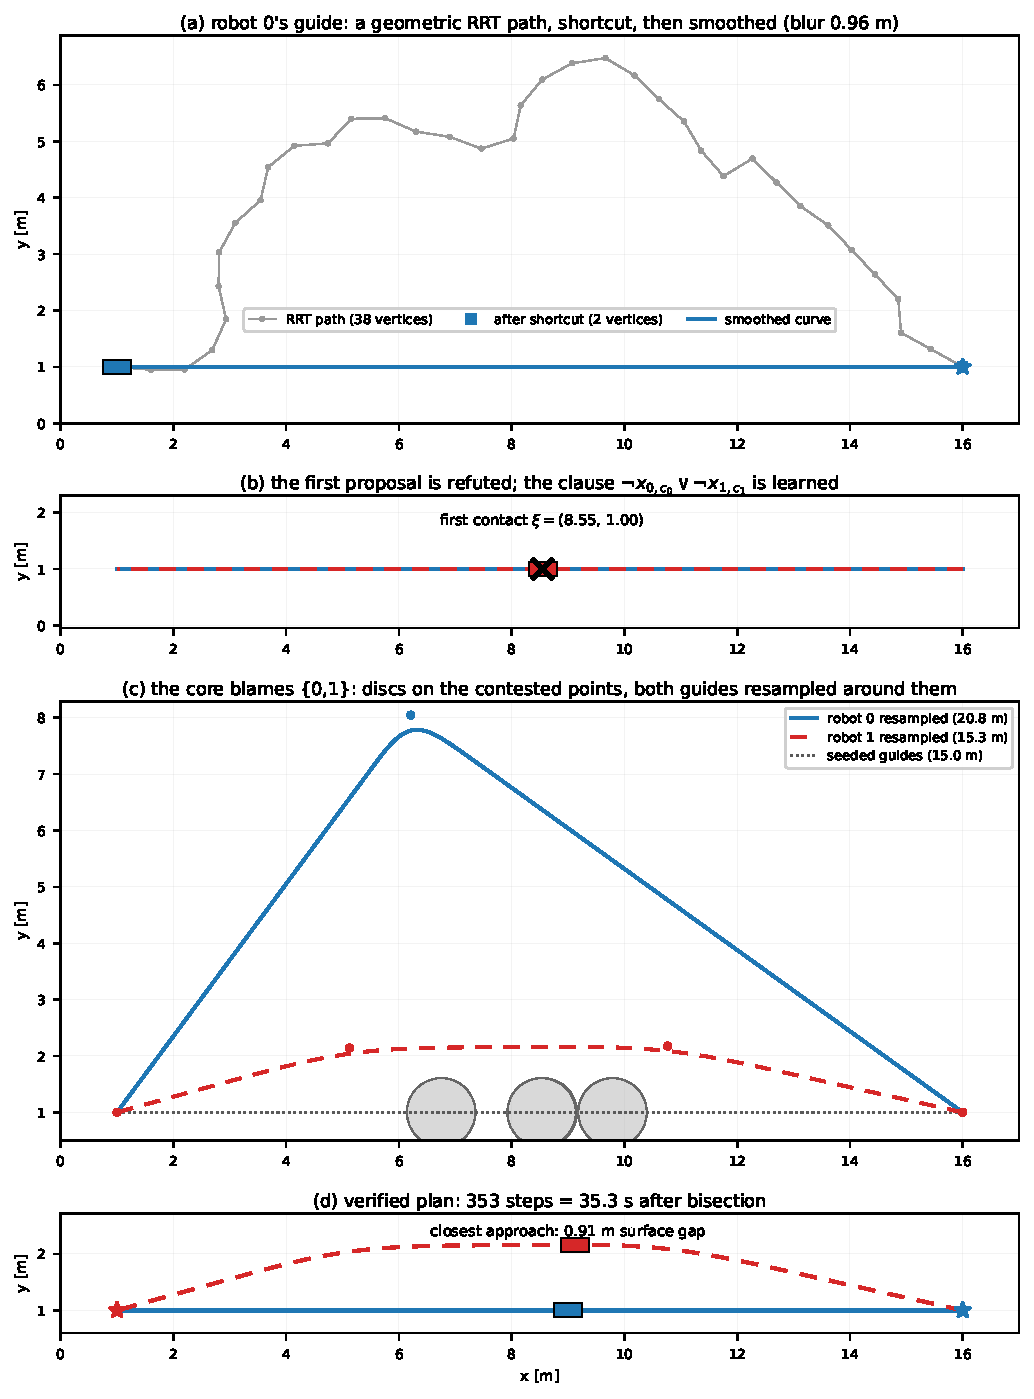
\includegraphics[width=0.86\textwidth]{figs/worked_example_cegar.pdf}
\caption{The loop on the lower row of \texttt{open\_cross\_4} (the upper row is resolved the
same way in round 2). Robot $0$ is blue and solid, robot $1$ red and dashed; starts are drawn
as bodies, goals as stars. Every panel is to scale.
\textbf{(a)} Robot $0$'s seed guide: the raw RRT path ($38$ vertices, grey) shortcuts to a
single segment (squares), and the smoothed curve with the largest admissible blur,
$\sigma^\ast = 0.96$\,m, lies on it.
\textbf{(b)} z3's first proposal is refuted: both robots meet at $\xi = (8.55, 1.00)$ (cross)
and a clause forbidding that pair of candidates is learned.
\textbf{(c)} After the core blames $\{0,1\}$, virtual obstacles of radius $b = 0.609$\,m are
placed on the contested points (grey discs; two of the four nearly coincide) and both robots are
resampled around them. Dots are the new guides' vertices, lines their smoothed curves.
\textbf{(d)} The verified plan after bisection: $353$ steps. Robot $0$ drives straight;
robot $1$ swerves around it; closest pass $0.91$\,m.}
\label{fig:worked}
\end{figure*}

This section runs the whole method on a small instance and reports the numbers the
implementation produced in one run.

\subsection{The instance}

The instance is \texttt{open\_cross\_4}, a four-robot version of the ``Open Cross'' benchmark
of \cite{karc2025}, in which the robots in each row swap ends across an empty room
(Table~\ref{tab:instance}). There are two rows $15$\,m apart, each with one head-on pair. The
rows are far enough apart never to interact, which is what makes the instance useful for
teaching: the correct blame is $\{0,1\}$ and $\{2,3\}$, never a mix, so we can check whether
the core finds it.

\begin{table}[t]
\caption{The worked instance, \texttt{open\_cross\_4}.}
\label{tab:instance}
\centering
\small
\begin{tabular}{ll}
\toprule
workspace $\W$ & $17.0 \times 17.0$\,m, no obstacles ($M = 0$) \\
robots $N$ & $4$, all \texttt{unicycle2\_v0} (Def.~\ref{def:robot}) \\
body $A_i$ & box $0.5 \times 0.25$\,m; $r^{+}=0.2795$, $r^{-}=0.125$\,m \\
robot $0$ & $(1,1) \rightarrow (16,1)$, $\theta^0 = 0$ \\
robot $1$ & $(16,1) \rightarrow (1,1)$, $\theta^0 = \pi$ \\
robot $2$ & $(1,16) \rightarrow (16,16)$, $\theta^0 = 0$ \\
robot $3$ & $(16,16) \rightarrow (1,16)$, $\theta^0 = \pi$ \\
$\Delta t$, $T_{\max}$ & $0.1$\,s; $1300$ steps ($130$\,s) \\
$\varrho$, $\clr$ & $0.2$\,m; $0.05$\,m \\
planner seed & $0$ \\
\bottomrule
\end{tabular}
\end{table}

\subsection{Seeding}

In an empty room the RRT still wanders: robot $0$'s raw tree path has $38$ vertices and climbs
to $y \approx 6.5$\,m before coming back down (Fig.~\ref{fig:worked}(a), grey). Shortcutting
removes every intermediate vertex, leaving the straight $15.000$\,m segment from start to
goal; the same happens for all four robots. On a straight guide every blur leaves the curve on
the guide, so \eqref{eq:fitblur} picks the largest, $\sigma^\ast = 0.96$\,m. The curvature is
zero, the cap \eqref{eq:vlim} is just $v_{\max}$, and the sweeps give a trapezoid: accelerate
for $2$\,s, cruise at $0.5$\,m/s, brake for $2$\,s.

\textsc{Variants} gives four candidates per robot. For robot $0$ their lengths are
\[
  \big(|\tau_0^{(0)}|,|\tau_0^{(1)}|,|\tau_0^{(2)}|,|\tau_0^{(3)}|\big) = (321,\ 513,\ 371,\ 421)
\]
steps: fastest; slowed by $\lambda = 1.6$; wait $30$ steps; wait $80$ steps. Each wait costs
its $w$ steps plus $20$ steps for the extra stop and restart. Robot $1$'s are
$(323, 515, 373, 423)$, and the upper row repeats the lower. So $|\Cand| = (4,4,4,4)$.

\subsection{Round 1: refute, prove, explain, repair}

z3's first proposal is refuted at once, on two pairs: robots $0$ and $1$ meet at
$\xi = (8.55,\ 1.00)$, and robots $2$ and $3$ at $(8.55,\ 16.00)$
(Fig.~\ref{fig:worked}(b)). Both robots of a row leave together at the same speed and meet near
the middle. Two clauses are learned,
\begin{align*}
  \ell_{0,c_0,1,c_1} &\rightarrow (\neg x_{0,c_0} \vee \neg x_{1,c_1}),\\
  \ell_{2,c_2,3,c_3} &\rightarrow (\neg x_{2,c_2} \vee \neg x_{3,c_3}),
\end{align*}
for the indices $c_0,\dots,c_3$ z3 happened to propose, and z3 proposes again.

It keeps proposing, and the oracle keeps refuting. Every one of the $4 \times 4 = 16$
combinations within the lower row conflicts, and so does every one within the upper row:
slowing one robot moves the meeting point along the row but does not remove it, and a wait only
shifts it. After $96$ pairwise checks, of which $32$ are refutations (all $16 + 16$ within-row
combinations; the other $64$ checks were between rows and clear), z3 reports \textsc{unsat}.

This is where the method departs from a conflict-driven planner. The message is not ``these two
touched'' but ``\emph{no} selection over $\Cand_0\times\Cand_1\times\Cand_2\times\Cand_3$ is
collision-free''. Every waiting and slowing option has been exhausted by the solver, without
generating anything new. The core blames exactly $\{0,1\}$. Its first four contested points,
which become the virtual obstacles, are
\[
  (8.55,1.00),\ (6.75,1.00),\ (8.53,1.00),\ (9.79,1.00),
\]
all on the lower row and spread along it --- the places where the pair meets under different
timings. (The first and third nearly coincide, so Fig.~\ref{fig:worked}(c) shows three discs.)
The upper row is not in this core. That is correct: its refutations are not needed to prove
that the lower row is stuck.

\textsc{Repair} resamples robots $0$ and $1$ around the discs. Robot $0$'s new guide has $3$
vertices and $20.83$\,m, a wide detour peaking near $y = 8$\,m; robot $1$'s has $4$ vertices and
$15.29$\,m, a gentle arc to $y \approx 2.2$\,m (Fig.~\ref{fig:worked}(c)). Each robot gets the four
variants of its new guide plus one $200$-step wait on its seed path, so $|\Cand| = (9,9,4,4)$.

\subsection{Round 2: the same proof, for free}

Round 2 performs \textbf{zero} new pairwise checks. With the new candidates the solver can now
satisfy the lower row, but the upper row is still ruled out entirely by the $16$ clauses cached
in round 1. z3 returns \textsc{unsat} straight away, with a core blaming $\{2,3\}$ and contested
points $(8.55,16),\ (6.75,16),\ (9.35,16),\ (7.29,16)$. Repair gives robot $2$ a $15.59$\,m guide
and robot $3$ a $17.71$\,m guide, and $|\Cand| = (9,9,9,9)$, $36$ candidates in total.

This round is the clearest illustration of Prop.~\ref{prop:monotone}: the geometric work of
round 1 was enough, on its own, to prove the next impasse.

\subsection{Round 3: satisfy, verify, shorten}

Round 3 needs $30$ more pairwise checks and finds $1$ more refutation, again at
$(8.55, 16.00)$; then z3's proposal passes every check and the verifier, at $T = 698$ steps.
That plan is long because z3 gave robot $0$ its $20.8$\,m detour, driven without waiting
($698$ steps); nothing in the rounds asks for a short plan, only a collision-free one.

Bisection starts from $T^\ast = 698$ and $T_{\text{lo}} = \max_i \min_c |\tau_i^{(c)}| = 323$.
The probes, in order, are:
\begin{center}
\small
\begin{tabular}{rll}
\toprule
cap $h$ & verdict & update \\
\midrule
$510$ & \textsc{sat}, $460$ steps & $T^\ast = 460$ \\
$391$ & \textsc{sat}, $371$ steps & $T^\ast = 371$ \\
$346$ & \textsc{unsat} & $T_{\text{lo}} = 347$ \\
$358$ & \textsc{sat}, $353$ steps & $T^\ast = 353$ \\
$349,\ 351,\ 352$ & \textsc{unsat} each & $T_{\text{lo}} = 353$ \\
\bottomrule
\end{tabular}
\end{center}
Bisection stops with $T_{\text{lo}} = T^\ast = 353$ after $7$ of the $12$ allowed probes, so
Prop.~\ref{prop:bisect} applies: no selection from these $36$ candidates finishes in $352$
steps. The reason is readable off the candidate lengths. Under a cap of $352$, neither robot $2$
(whose new candidates take $353$ steps or more) nor robot $3$ ($528$ or more) can use its new
guide, and the $200$-step waits are far too long, so each is left with its fastest seed
candidate --- a combination refuted in round 1. The makespan went from $698$ to $353$ steps ($-49\%$) without generating a single new
candidate.

The returned plan is in Fig.~\ref{fig:worked}(d) and Table~\ref{tab:result}. In each row
\emph{one} robot drives the straight seed path at full speed and the other swerves around it,
also at full speed: no robot waits, and no robot slows. Which robot yields is a choice the
solver made (robot $1$ in the lower row, robot $2$ in the upper row); no priority rule
produced it.

\begin{table}[t]
\caption{The returned plan. Excursion is the largest distance from the straight line between
start and goal; arrival is the first time within $\varrho$ of the goal.}
\label{tab:result}
\centering
\small
\begin{tabular}{lrrrrr}
\toprule
robot & excursion & arrival & path len. & $\max|v|$ & $\max|\omega|$ \\
      & [m] & [s] & [m] & [m/s] & [rad/s] \\
\midrule
$0$ & $0.000$ & $30.7$ & $14.999$ & $0.500$ & $0.000$ \\
$1$ & $1.164$ & $33.2$ & $15.253$ & $0.500$ & $0.221$ \\
$2$ & $1.916$ & $33.9$ & $15.509$ & $0.500$ & $0.257$ \\
$3$ & $0.000$ & $30.9$ & $15.000$ & $0.500$ & $0.000$ \\
\midrule
\multicolumn{6}{l}{makespan $35.3$\,s ($353$ steps); verified by the simulator's checker}\\
\multicolumn{6}{l}{closest pass: pair $(0,1)$ $0.914$\,m at step $169$; pair $(2,3)$ $1.599$\,m}\\
\bottomrule
\end{tabular}
\end{table}

\begin{table}[t]
\caption{Round-by-round trace of the worked instance. ``checks'' and ``refut.'' are
cumulative. Round~2 performs no geometric work at all.}
\label{tab:rounds}
\centering
\small
\setlength{\tabcolsep}{4pt}
\begin{tabular}{crrcl}
\toprule
rnd & checks & refut. & blamed & $|\Cand|$ after repair \\
\midrule
$1$ & $96$  & $32$ & $\{0,1\}$ & $(9,9,4,4)$ \\
$2$ & $96$  & $32$ & $\{2,3\}$ & $(9,9,9,9)$ \\
$3$ & $126$ & $33$ & --- & \textsc{sat}, $T\!=\!698 \rightarrow 353$ (certified) \\
\bottomrule
\end{tabular}
\end{table}


\subsection{What the example shows}

\begin{itemize}
  \item \textbf{The core localises correctly.} On an instance with known structure, the core
        named exactly the stuck pair in each round, without being told the rows were
        independent.
  \item \textbf{New geometry is only generated when proved necessary.} Before any resampling,
        the solver ruled out all $16$ timing combinations per row using the slowed and waiting
        variants already present.
  \item \textbf{Learned clauses are reused.} Round 2 proved a second impasse with zero new
        checks, and bisection certified the makespan using round-1 refutations.
  \item \textbf{The solver chooses who yields.} There is no priority order in the method.
\end{itemize}

\section{Why These Standard Components}
\label{sec:design}

We kept the candidate generator as conventional as possible, but each component is there for
a measured reason. The measurements below are single runs (the planner is randomised; see
Sec.~\ref{sec:limits} on variance), so they indicate size of effect, not a statistic.

\paragraph*{Why not kinodynamic RRT candidates}
A kinodynamic RRT samples controls and so cannot aim at a state (Remark~\ref{rem:steer}). On a
single robot crossing $15$\,m of empty room with goal tolerance $0.2$\,m, a control-sampling
RRT had its closest node at $1.612$\,m from the goal after $1000$ iterations ($5.4$\,s) and
still $1.612$\,m after $3000$ ($18.2$\,s); relaxing the tolerance to $1.0$\,m did not change
this. It gets close and cannot close the gap, and a candidate that does not reach the goal is
useless to the selection problem.

\paragraph*{Why a smooth traverse rather than stop-and-turn}
The simplest drivable realisation of a polyline is rest-to-rest: at each vertex, stop, turn on
the spot, accelerate along the next segment. Replacing \textsc{Drive} with that, everything
else unchanged:
\begin{center}
\small
\setlength{\tabcolsep}{3.5pt}
\begin{tabular}{lcc}
\toprule
scenario & smooth (ours) & stop-and-turn \\
\midrule
\texttt{cluttered\_cross\_16} & $711$ steps, $11.0$\,s & $1031$ steps, $32.5$\,s \\
\texttt{open\_cross\_32} & $537$ steps, $102.3$\,s & \textsc{fail} at $619$\,s \\
\bottomrule
\end{tabular}
\end{center}
Longer candidates overlap in time with more of the other robots' candidates, which means more
refutations ($203$ vs.\ $98$ on the first row), more rounds, and on $32$ robots a candidate
supply that never catches up.

\paragraph*{Why search the blur}
Using the base blur $\sigma_0 = 0.12$\,m everywhere instead of \eqref{eq:fitblur}:
\texttt{cluttered\_cross\_16} $991$ vs.\ $711$ steps and \texttt{open\_cross\_32} $722$ vs.\
$398$ steps, at essentially the same wall time. ($398$ here and $537$ in the previous table are
two runs of the identical configuration; the difference is run-to-run variance.) The blur search does not decide
\emph{whether} a plan is found; it decides how fast the robots drive (Prop.~\ref{prop:caps}).

\section{Experimental Evaluation}
\label{sec:experiments}

\paragraph*{Setup}
We use ports of the Open Cross and Cluttered Cross scenarios of \cite{karc2025}, with
$N \in \{16, 32\}$
second-order unicycles (Def.~\ref{def:robot}), start states fixed per scenario, and $5$
planner seeds per cell; seeds change the planner's random numbers, not the instance. The
budget is $600$\,s per run. The scenarios are ports from the published description, not
reproductions: \cite{karc2025} gives no workspace dimensions, clearance, time step or velocity
limits, so ours are the values of Table~\ref{tab:instance} and Def.~\ref{def:robot}. A run counts as a success only if the plan, executed in the
simulator, reaches every goal with zero collisions. Wall time is Python on one machine and is
not comparable to published C++ numbers.

\begin{table}[t]
\caption{Core-guided resampling over $5$ seeds. Steps and wall time are over successful seeds
(median, with range). \texttt{open\_16} abbreviates \texttt{open\_cross\_16}, etc.}
\label{tab:results}
\centering
\small
\setlength{\tabcolsep}{2.5pt}
\begin{tabular}{lccc}
\toprule
scenario & succ. & steps & wall [s] \\
\midrule
\texttt{open\_16}      & $5/5$ & $361$ ($355$--$441$) & $25.1$ ($18.7$--$601.1$) \\
\texttt{open\_32}      & $4/5$ & $526.5$ ($500$--$531$) & $67.8$ ($56.0$--$84.1$) \\
\texttt{cluttered\_16} & $5/5$ & $639$ ($593$--$691$) & $19.6$ ($11.4$--$159.2$) \\
\texttt{cluttered\_32} & $3/5$ & $617$ ($607$--$635$) & $129.0$ ($84.2$--$617.7$) \\
\bottomrule
\end{tabular}
\end{table}

\paragraph*{Results}
Table~\ref{tab:results} reports our method alone. Of the $20$ runs, $17$ succeeded. Two failed
by exhausting the budget (\texttt{open\_cross\_32} and \texttt{cluttered\_cross\_32}, one seed
each). The third failure, on \texttt{cluttered\_cross\_32}, is a plan the planner verified but
the simulator's rollout scored with $13$ collision steps; it is counted as a failure here and
discussed in Sec.~\ref{sec:limits}. Wall time is typically well under a minute at $N = 16$ and
around one to two minutes at $N = 32$, with a long tail: two successful runs finished only
just past the $600$\,s budget.

\paragraph*{Comparison with K-ARC}
\emph{[Pending: the K-ARC baseline over the same cells is still running and will be reported
here under identical conditions. No comparison is claimed until it completes.]}

\section{Limitations}
\label{sec:limits}

\paragraph*{Discrete-time collision semantics}
Stated in Remark~\ref{rem:gap}; it has known fixes.

\paragraph*{Planned versus executed goal behaviour}
The verifier assumes a robot keeps following its candidate until that candidate ends at rest
on its goal. The simulator instead parks a robot the moment it is inside $\varrho$ below a
stopping speed, which can be a short distance before the planned stopping point. On one of our
$20$ runs the simulator scored collisions on a plan the verifier had accepted; this mismatch is
our leading explanation and is being confirmed by replay. The fix is to verify under the
simulator's parking rule (or disable it); until then,
Prop.~\ref{prop:sound} holds for the plan as planned, and the experiments count such runs as
failures.

\paragraph*{Variance and nondeterminism}
The planner is randomised, and z3's choice among satisfying assignments also depends on
internal state. Repeated runs of one configuration on \texttt{open\_cross\_32} produced $398$,
$516$ and $537$ steps. Every number in Sec.~\ref{sec:example} comes from one run in a fresh
process, and every number in Sec.~\ref{sec:design} is a single run.

\paragraph*{Resampling can overshoot}
The sampler is not asked for a short detour, only an unobstructed one. In the worked example
robot $0$'s repair path was $20.8$\,m for a $15$\,m crossing. The solver did not use it ---
bisection found a better selection --- but on crowded instances such candidates cost rollout
and checking time.

\paragraph*{Robots in a core are repaired independently}
Each blamed robot is resampled on its own. When the resolution an instance needs is a shared
convention --- all robots passing a junction on the same side --- independent resampling can push
two blamed robots into each other's new corridor. A joint repair of a whole core is the natural
next step, and one a pairwise trigger cannot express, since it never has more than two robots in
scope.

\paragraph*{Budget overrun}
The deadline is checked between solver calls only (we observed up to $18$\,s of overrun).

\section{Conclusion}

We presented a multi-robot kinodynamic planner in which the decision to generate new motion is
triggered by a proof rather than by an observed collision. Candidate motions are built from
standard parts --- a geometric RRT, shortcutting, corner smoothing, a speed profile and a
tracking rollout --- so each is drivable by the robot on its own. A SAT solver selects among
them under lazily learned conflict clauses; when it proves that no selection works, the
unsatisfiable core names the robots that are stuck and the points where they are stuck, and
only those robots are resampled, away from those points. The same clause database lets one
round's refutations prove the next round's impasse, and turns horizon bisection into a
certificate that the returned makespan is the best the candidates allow.

\section*{Reproducibility}

The worked instance is \texttt{conf/env/open\_cross\_4\_unicycle2.yaml} with
\texttt{approach.method=cegar}. Fig.~\ref{fig:worked} and every number in
Sec.~\ref{sec:example} are printed by \texttt{scripts/worked\_example\_cegar\_fig.py} (seed
$0$, fresh process). Table~\ref{tab:results} is produced by \texttt{scripts/karc\_bench.py
--methods cegar --seeds 0 1 2 3 4}.

\section*{Disclosure}

Portions of the software and of this manuscript were prepared with the assistance of a large
language model. All experimental results were produced by the authors' own code and verified by
the authors; all citations were checked against their primary records before inclusion.

\bibliographystyle{IEEEtran}
\bibliography{refs}

\end{document}
